\chapter{Molekülphysik}
\label{chap:molekuelphysik}
\clearpage
\section{Einführung}

\begin{verbal}
    Die Themen der Molekülphysik sind vielseitig: während einfache Moleküle heute gut verstanden sind, widmet sich die heutige Forschung vor allem dynamischen Systemen. In dieser Vorlesung soll es jedoch um einfache Moleküle mit wenigen Atomen gehen.
\end{verbal}
    \subsection{Motivation}
    \paragraph{Ziele der Vorlesung} Wir wollen verstehen...
    \begin{itemize}
    	\item wieso gibt es $\text{H}_{2}$ aber kein $\text{H}_{3}$ 
    	\item wieso ist $\text{NH}_{3}$ eine Pyramide?
    	\item wieso ist $\text{CH}_{4}$ ein Tetraeder?
    	\item wieso ist $\text{C}_{6} \text{H}_{6}$ (Benzol) flach?
    	\item wie sind Moleküle aufgebaut?
    	\item welche Kräfte halten Moleküle zusammen?
    		\begin{center}
    			$\text{O}_{2}$ (kovalent) vs. $\text{KBr}$ (ionisch)
    		\end{center}
    	\item wie groß und schwer sind Moleküle?
    	\item was sind die elektrischen und magnetischen Eigenschaften von Molekülen?
    	\item können wir die komplexen optischen Spektren von Molekülen verstehen und zur Beantwortung obiger Fragen nutzen?
    \end{itemize}
    \paragraph{Aktuelle Forschung} Aktuelle Fragen in der Forschung sind in der...
    \begin{itemize}
    	\item Umwelttechnik: Fernanalyse von Schadstoffen und Emissionen, Ozonloch, Treibhauseffekt ($\text{CO}_{2}$, $\text{H}_{2}\text{O}$)
    	\item Astrophysik: Atmosphäre von Planeten, Gibt es Leben außerhalb der Erde?
    	\item Biologie: Proteine, Makromoleküle
    \end{itemize}
    
    \paragraph{Unterschiede zur Atomphysik} Wesentliche Unterschiede zur Atomphysik sind
    \begin{itemize}
    	\item Innere Freiheitsgrade vorhanden (Rotation, Schwingung)
    	\item Größere Mannigfaltigkeit: 
    		\begin{itemize}
    			\item Einfache Moleküle ($\text{H}_{2}$, $\text{O}_{2}$, $\text{HCl}$...)
    			\item Große Moleküle ($\text{C}_{6}\text{H}_{6}$)
    			\item Makromoleküle ($\sim $ 1000 Atome, Polyacetylen)
    			\item Biomoleküle (DNS (engl. DNA))
    		\end{itemize}
    	\item Wirkung in Physik, Chemie, Biologie
    \end{itemize}
    \begin{verbal}
        Biomoleküle werden meist in Spezialvorlesungen der Physik und Chemie, sowie bei Vorlesungen der (technischen) Biologie betrachtet.
    \end{verbal}
    
    \paragraph{Historische Bemerkungen} Die Molekülphysik hat bereits eine lange Historie. Wichtige Ecksteine sind
    \begin{itemize}
    	\item \textbf{1811 Avogadro}: Einführung des Begriffs Molekül im Zusammenhang mit chemischen Reaktionen.\\
    		Hypothese: Gleiche Volumina verschiedener idealer Gase enthalten bei gleicher Temperatur und gleichem Druck gleich viele Moleküle oder Atome
    	\item \textbf{1864 Kékule:} Entdecker der Benzolstruktur
    	\item \textbf{Loschmidt:} Berechnung von Zahlenwerten für die Größe von Molekülen mit Hilfe der kinetischen Gastheorie
    	\item \textbf{20. Jahrhundert Kossel:} heteropolare Bindung
    	\item \textbf{1915-1920 Lewis und Langmuir:} homöopolare Bindung
    	\item \textbf{Hund, Heitler, London und andere:} Quantentheorie der chemischen Bindung
    	\item \textbf{NP 1954 Linus Pauling:} Natur der chemischen Bindung und ihre Anwendung zur Aufhellung der Struktur komplexer Substanzen 
    	\item \textbf{1960 Crick und Watson:} Doppelhelix der DNA-Struktur
    	\item \textbf{NP 1988 Michel, Huber, Dreisenhofer:} 3D-Struktur des photsynthese Reaktionszentrums
    	\item \textbf{NP 1996 Curl, Kroto, Smalley:} $\text{C}_{60}$ (3. Modifikation des Kohlenstoffs) ($\text{sp}^{2}$, $\text{sp}^{3}$)
    	\item \textbf{NP 2002 Fenn, Tanaka, Wüthrich:} Analyse von biologischen Makromolekülen
    	\item \textbf{NP 2008 Shimomura, Chalfie, Tsien:} Entdeckung und Weiterentwicklung des grün fluoreszierenden Proteins
        \item \textbf{NP 2024 Baker, Hassabis, Jumper: } Vorhersage und Gestaltung von Proteinstruktur mit künstlicher Intelligenz
    \end{itemize}

\subsection{Eigenschaften eines Moleküls}
    \subsubsection{Größe}
    Die Größe von Molekülen wurde im Laufe der Zeit mit unterschiedlichen Methoden gemessen, bzw. abgeschätzt.
    \paragraph{Avogadros Gesetz} ein Mol eines idealen Gases nimmt bei Normalbedingungen ein Volumen  von $\SI{22,4}{\liter}$ ein. Ein Mol besteht aus $N_{\text{A}} = 6,022 \cdot 10^{23}$ Molekülen.\\[1ex]
    Beim Phasenübergang Gas $\to$ Flüssigkeit, bzw. Gas $\to$ Festkörper nimmt das Volumen stark ab: beispielsweise ist das Volumen eines Festkörpers $\approx\frac1{1000}$ des Gasvolumens.\\
    $\to$ Annahme: Die Moleküle berühren sich.\\
    $\to $ Molekülradien $\sim \SI{1}{\angstrom}$
    
    \paragraph{$\bm{p}$-$\bm{V}$-Isothermen reeler Gase} $n=\SI{1}{\mol}$ eines reelen Gases wird mit 
        \begin{equation}
            \label{1.1}
            \left( p + \frac{a}{V^2} \right) \left( V-b \right) = RT
        \end{equation}
        beschrieben. Dazu wird der Binnendruck $a$ und das Kovolumen der Gasmoleküle $b$ verwendet, welches das etwa vierfache deren Eigenvolumens beträgt.
    \paragraph{Transportphänomene:}
        Gaskinetische Methoden (Diffusion, Viskosität, Wärmeleitung)
        \begin{itemize}[label=$\to$]
            \item mittlere freie Weglängen $\to $ Wirkungsquerschnitt
            \item Moleküldurchmesser (Haken-Wolf)
        \end{itemize}
    \paragraph{Moderne Methoden:}
        \begin{itemize}
            \item Transmissionselektronenmikroskopie (TEM)\\ Auflösungsgrenze $\sim \SI{0,05}{\nano\meter}$
            \item Rastersondenmikroskopie (STM, AFM)
        \end{itemize}
    
    \paragraph{Definition der Größe} Wenn man von der Größe $d$ eines Moleküls spricht, muss man definieren, um welche physikalischen Eigenschaften es sich handelt. Beispielsweise kann \begin{itemize}
        \item $d_\text{min}$ als der Abstand zweier Moleküle , an welchem die Energie minimal ist,
        \item $d_\text T$ als der Abstand, an welchem sich die Moleküle verformen,
    \end{itemize} 
    definiert werden. \autoref{fig:I.2_definiton_von_d} zeigt diese beiden Größen im radialabhängigen Potential. 
    
    \begin{figure}[H]
        \centering
        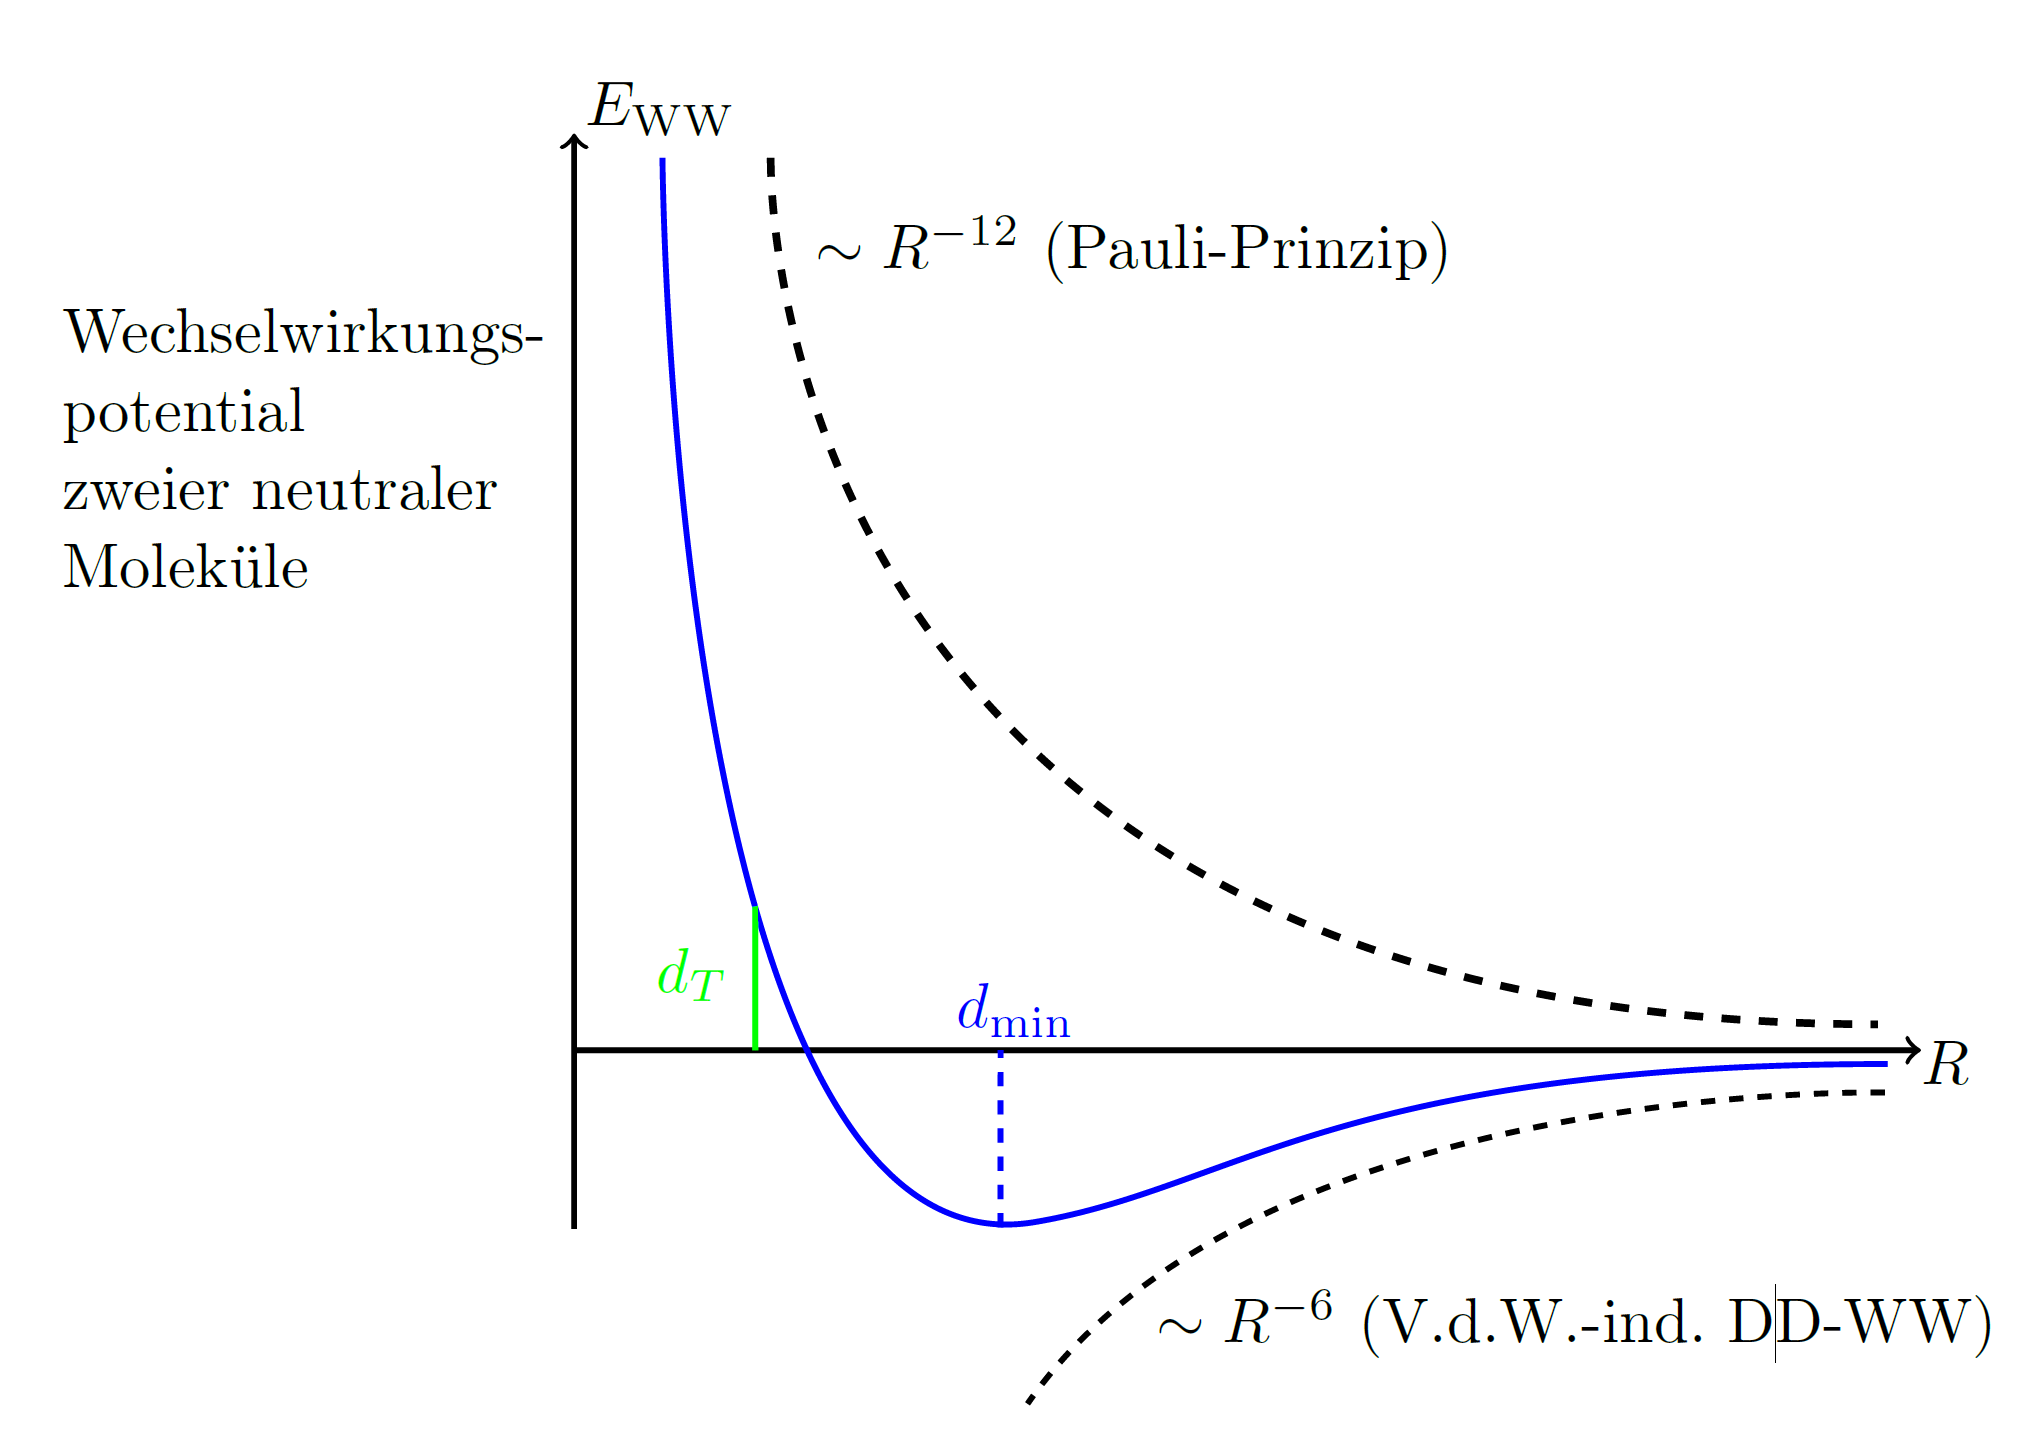
\includegraphics[width=0.8\linewidth]{figures/vl01/definition_von_d.png}
        \caption{Minimaler Abstand $d_\text{min}$ und Verformungsabstand $d_\text{T}$ zweier Moleküle. Blau eingezeichnet ist das Wechselwirkungspotential zwischen den Molekülen, welches sich aus einem abstoßendem Potential $\sim R^{-12}$ nach dem Pauli-Prinzip und einem attraktiven Potential $\sim R^{-6}$ nach der Van-der-Waals-induzierten Wechselwirkung (V.d.W.-ind. DD-WW) zusammensetzt.}
        \label{fig:I.2_definiton_von_d}
    \end{figure}
    
    
    \subsubsection{Form}
        Über die Form von Molekülen können durch verschiedene Verfahren Informationen gewonnen werden. Unter anderem kann durch...
        \begin{itemize}
        	\item \textbf{Röntgen, Neutronen-, und Elektronenbeugung} an geordneten Strukturen die Abstände zwischen Kernen auf $\pm\SI{0,01}{\angstrom}$ und der Winkel auf $\SI{0,01}{\degree}$ bestimmt werden.
        	\item \textbf{Spektroskopie} das Spektrum eines Moleküls analysiert werden.
        \end{itemize}
    
    \subsubsection{Masse}
        \begin{verbal}
            Die Massenbestimmung ist im Haken-Wolf beschrieben. In dieser Vorlesung soll sie nicht besprochen werden.
        \end{verbal}
    
\subsubsection{Spez. Wärme und kinetische Energie}
    Experimentell zeigt sich, dass die spezifische Wärmekapazität eines Stoffes von seiner Temperatur abhängt. Für das Wasserstoffmolekül H${}_2$ ist dieser Verlauf in \autoref{fig:I.2_spez_waerme_u_kin_E} dargestellt.
    \begin{figure}[H]
        \centering
        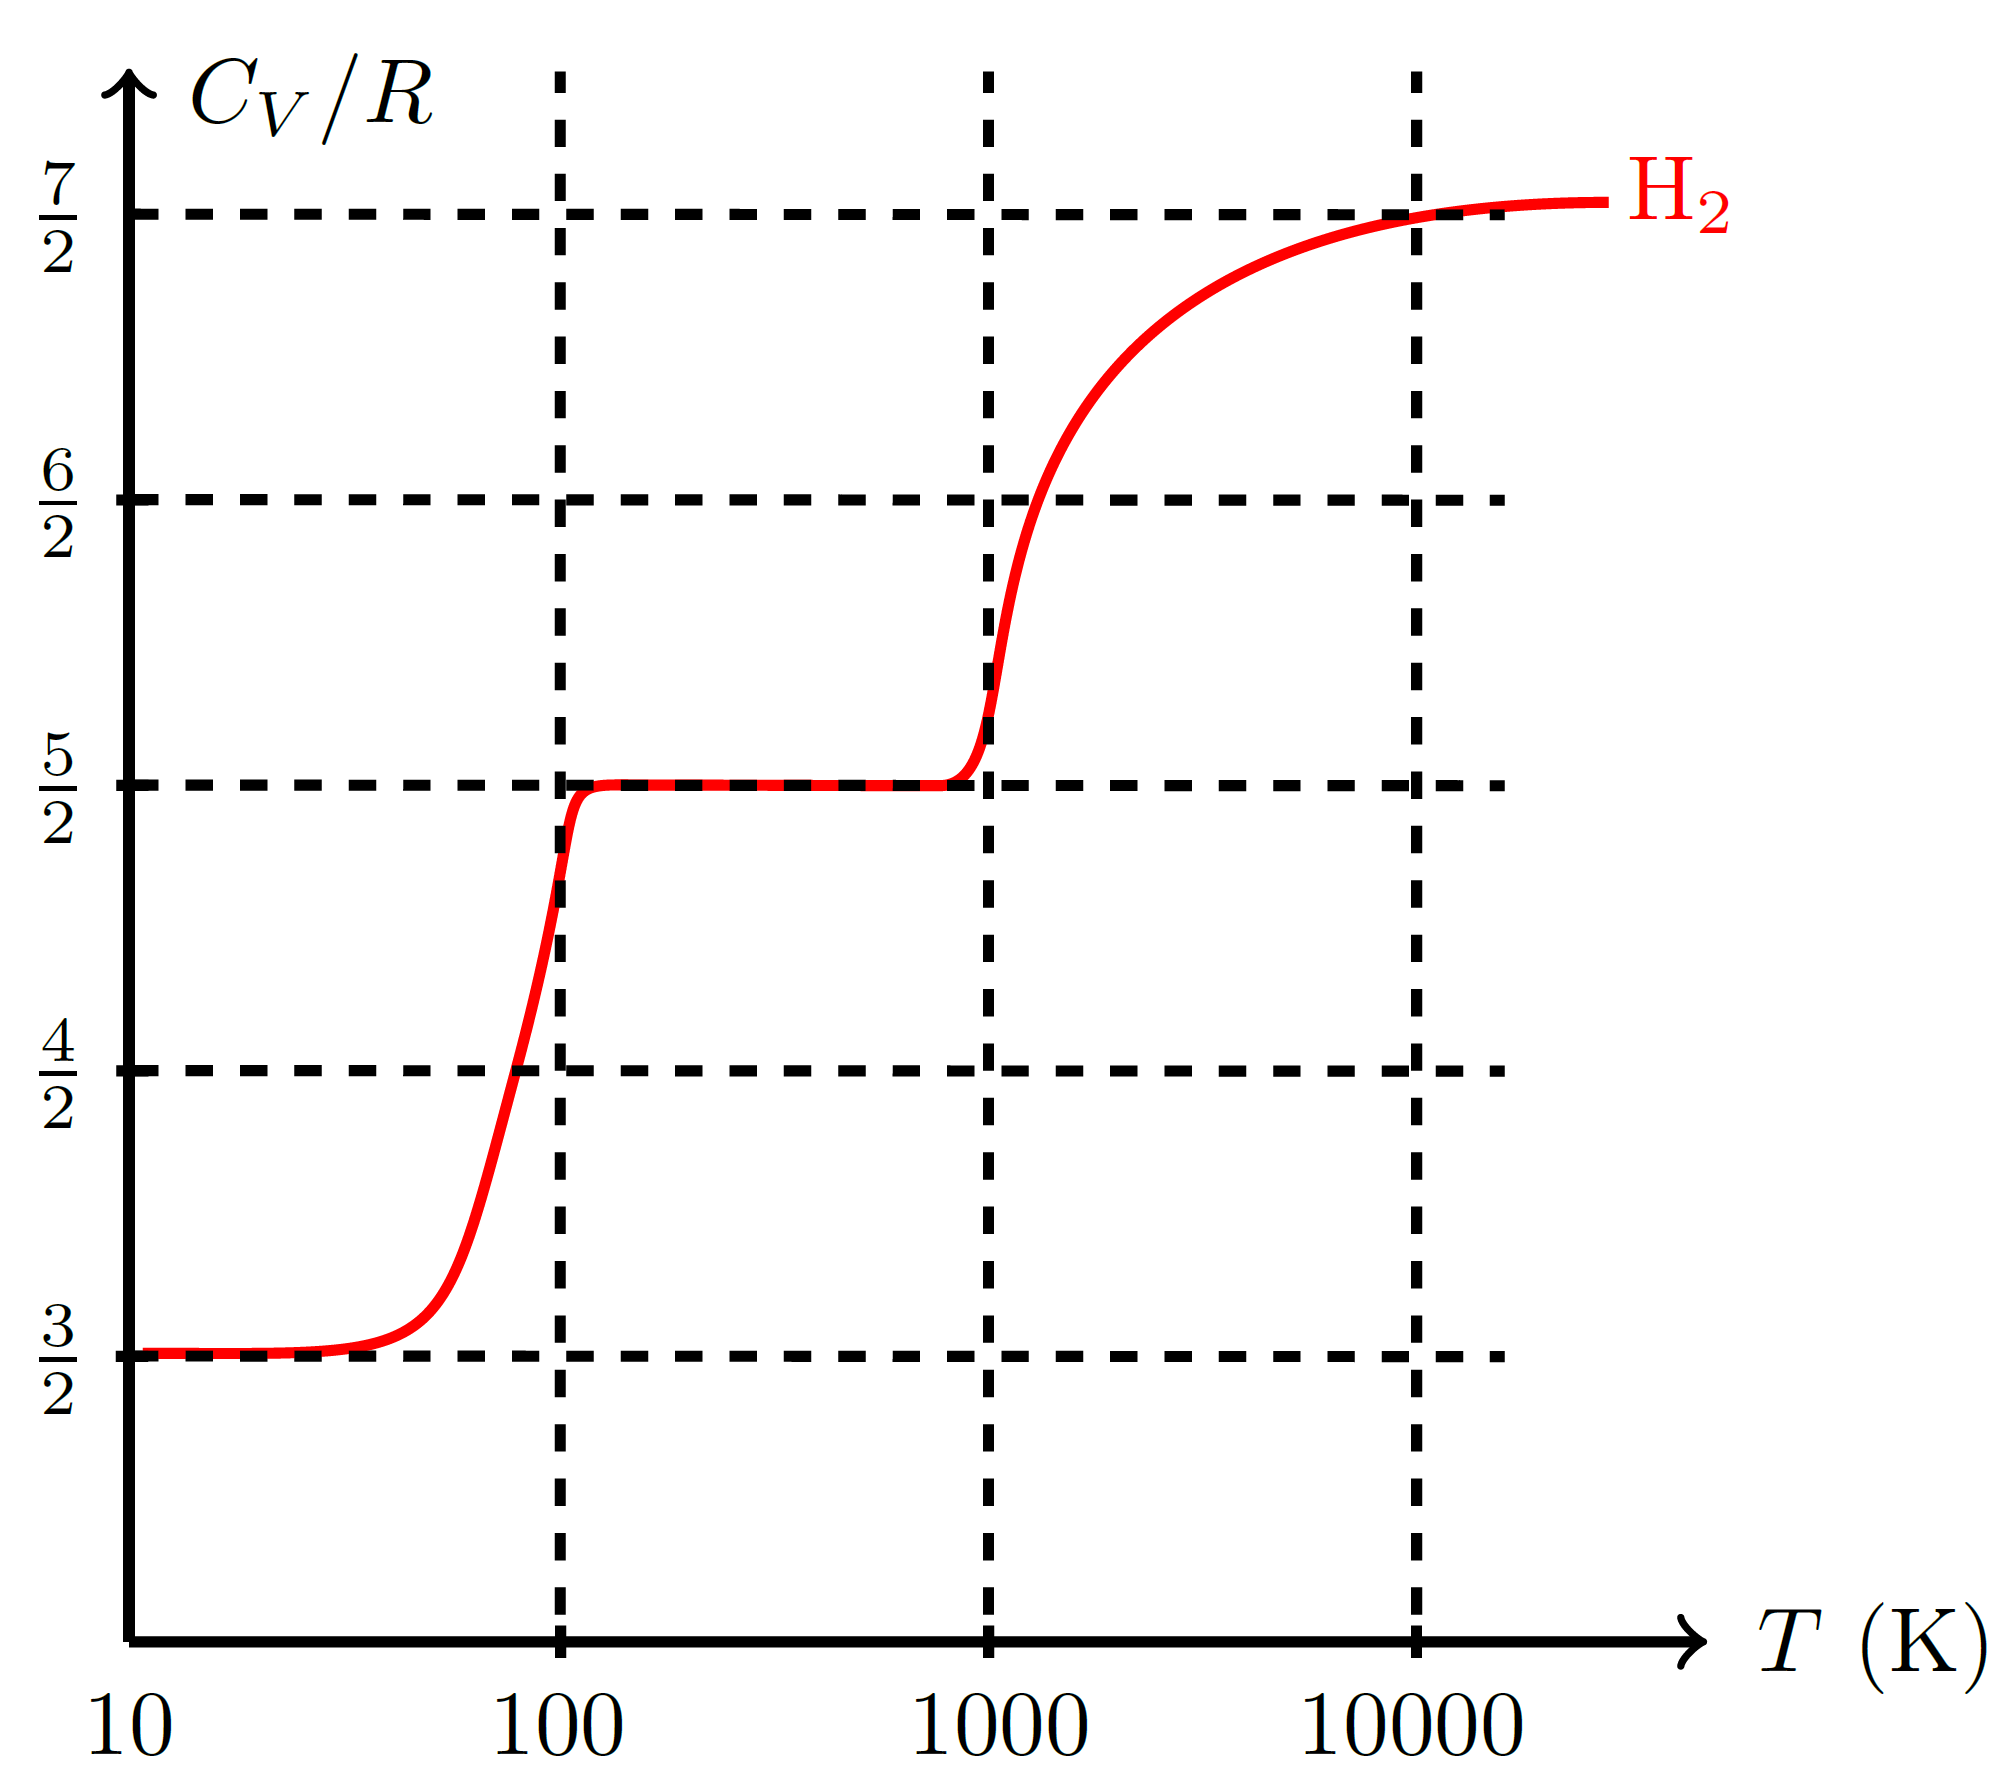
\includegraphics[width=0.6\linewidth]{figures/vl01/spez_waerme_u_kin_E.png}
        \caption{Spezifische Wärmekapazität $C_\text V/R$ von Wasserstoff H${}_2$ aufgezeichnet über die Temperatur $T$.}
        \label{fig:I.2_spez_waerme_u_kin_E}
    \end{figure}
\paragraph{Spezifische Wärmekapazität}
    Die Wärmekapazität gibt Rückschlüsse auf die Anzahl und die Bewegungsstände der Moleküle:
    Ein Molekül mit drei Freiheitsgraden der Translation hat die kinetische Energie
    $$
    \bar{E}_{\text{kin}} = \frac{3}{2} k_{B}T.
    $$
    Ein Mol diesen Stoffes hat die kinetische Energie
    $$\bar{E}_{\text{kin}}^{\text{mol}} =\frac{3}{2} \mathrm{N}_{\mathrm{A}}\mathrm{k}_\mathrm{B} T = \frac{3}{2} RT
    $$
    Ein einzelner Freiheitsgrad $f$ hat die kinetische Energie
    $$
    \bar{E}_{\text{kin}, f} = \frac{1}{2} k_{B}T
    $$
    Die spezifische Wärmekapazität ist definiert als die Temperaturableitung der Energie
    $$
    C_{V}^{\text{Mol}} = \frac{\text{d}\bar{E}}{\text{d}T} = \frac{3}{2} R \quad \to \quad  C_{V}^{\text{Mol}} = \frac{f}{2} R
    $$

\paragraph{Temperaturabhängigkeit der spezifischen Wärmekapazität} 
    Bei Molekülen hängt die spezifische Wärmekapazität $C_{V}$ von der Temperatur $T$ ab (vgl. $\text{H}_{2}$ in \autoref{fig:I.2_spez_waerme_u_kin_E}).\par
    
    Ein Molekül hat \textbf{innere} Freiheitsgrade, die mit der Rotation und Schwingung verknüpft sind. Energiezustände sind gequantelt und verschieden groß.
    \begin{itemize}
    	\item \textbf{Rotation:} $\frac{1}{2} \mathrm{k}_\mathrm{B} T $ pro Freiheitsgrad $f$, außer um die Längsachse bei linearen Molekülen wegen des kleinen Trägheitsmoments. Allgemein besitzen Moleküle jedoch 3 Rotationsfreiheitsgrade um die Hauptträgheitsachsen.
    	\item \textbf{Schwingung:} Atome im Molekül schwingen. Die Zahl der Freiheitsgrade 
        \begin{equation}
            f=3n-6
            \label{eq:I.2_schwingungs_freiheitsgrade}
        \end{equation}
        (bzw. $f=3n-5$ bei linearen Molekülen) hängt von der Atomzahl $n$ ab. Zweiatomige Moleküle ($n=2$) haben somit $f=1$ Schwingungsfreiheitsgrad.\\

    	Gleichung \eqref{eq:I.2_schwingungs_freiheitsgrade} folgt daraus, dass jedes Atom $f=3n$ Freiheitsgrade der Translation besitzt. Davon werden subtrahiert
        \begin{itemize}
        	\item 3 Freiheitsgrade der Translation des SP
        	\item 3 (2 für lineare) Freiheitsgrade der Rotation um die Hauptträgheitsachsen
        \end{itemize}
        \begin{verbal}
            Bei der Betrachtung von \autoref{fig:I.2_spez_waerme_u_kin_E} fällt auf, dass Wasserstoff scheinbar zwischen $\SI{1000}{\kelvin}$ und $\SI{10000}{\kelvin}$ zwei Freiheitsgrade dazubekommt. Das steht aber im Widerspruch dazu, dass nur ein Schwingungsfreiheitsgrad dazukommt.
        \end{verbal}
        Bei Freiheitsgraden der Schwingungen beträgt die Energie
        $$
        E = 2 \cdot \frac{1}{2} \mathrm{k}_\mathrm{B} T = \mathrm{k}_\mathrm{B}T
        $$ 
        pro Freiheitsgrad $f$, da sowohl potentielle, als auch kinetische Energie vorhanden sind.
        \end{itemize}

